\begin{lpu}
Maschinelles Lernen basiert auf Daten – und wer mit Daten arbeitet, braucht Statistik. Viele Verfahren des ML beruhen auf grundlegenden Begriffen der beschreibenden Statistik, z.\,B. wenn es darum geht, wie stark sich Werte unterscheiden oder wie ``typisch'' ein Wert ist.

Dieses Kapitel hat zwei Ziele:
\begin{itemize}
  \item Sie lernen zentrale statistische Begriffe kennen, die im ML immer wieder verwendet werden.
  \item Sie vertiefen Ihr Verständnis der bisher kennengelernten Algorithmen und lernen, sie sinnvoll voneinander zu unterscheiden.
\end{itemize}

Keine Angst, die meisten Begriffe hier kennen Sie bereits aus dem Mathematik-Unterricht. Den Einstieg macht hier eine kleine Repetition:

\begin{theorie}
\textbf{Die 3 M: Mittelwert, Median, Modus}. Um eine Zahlenreihe zusammenzufassen, gibt es drei klassische \textit{Lagekennwerte}:

\begin{itemize}
  \item Der \textbf{Mittelwert (arithmetisches Mittel)} gibt an, \emph{wo im Durchschnitt} die Werte liegen.
    \[
    \bar{x} = \frac{1}{n} \sum_{i=1}^{n} x_i
    \]

  \item \textbf{Median:} Der mittlere Wert, wenn die Zahlen sortiert sind. Bei ungerader Anzahl: der Wert in der Mitte. Bei gerader Anzahl: Durchschnitt der zwei mittleren Werte.

  \item \textbf{Modus:} Der Wert, der am häufigsten vorkommt.
\end{itemize}
\end{theorie}

Nehmen wir zum Beispiel die Zahlen $[92,\ 92,\ 88,\ 81,\ 56,\ 89,\ 90,\ 86,\ 93]$, oder in sortierter Reihenfolge:

\begin{center}
$[56,\ 81,\ 86,\ 88,\ 89,\ 90,\ 92,\ 92,\ 93]$
\end{center}

Damit können wir nun die 3 M berechnen:
\begin{itemize}
  \item Mittelwert: $\bar{x} = \frac{757}{9} \approx 84.1$
  \item Median: $89$ (5. Wert in sortierter Liste)
  \item Modus: $92$ (kommt zweimal vor)
\end{itemize}

\begin{figure}[h]
\centering
\begin{tikzpicture}[scale=0.3]
% Zahlenstrahl
\draw[->] (50,0) -- (100,0) node[right] {Werte};

% Ticks und Werte über dem Strahl
\draw (56,0) -- (56,0.5);
\node[above, yshift=0.8ex] at (56,0) {56};
\draw (81,0) -- (81,0.5);
\node[above, yshift=0.8ex] at (81,0) {81};
\draw (86,0) -- (86,0.5);
\node[above, yshift=0.8ex] at (86,0) {86};
\draw (88,0) -- (88,1.5);
\node[above, yshift=2.8ex] at (88,0) {88};
\draw (89,0) -- (89,0.5);
\node[above, yshift=0.8ex] at (89,0) {89};
\draw (90,0) -- (90,1.5);
\node[above, yshift=2.8ex] at (90,0) {90};
\draw (92,0) -- (92,0.5);
\node[above, yshift=0.8ex] at (92,0) {92};
\draw (93,0) -- (93,1.5);
\node[above, yshift=2.8ex] at (93,0) {93};

% Datenpunkte
\filldraw[black] (56,0) circle (3.5pt);
\filldraw[black] (81,0) circle (3.5pt);
\filldraw[black] (86,0) circle (3.5pt);
\filldraw[black] (88,0) circle (3.5pt);
\filldraw[black] (89,0) circle (3.5pt);
\filldraw[black] (90,0) circle (3.5pt);
\filldraw[black] (92,0) circle (3.5pt);
\filldraw[black] (92,0) circle (3.5pt);
\filldraw[black] (93,0) circle (3.5pt);

% Mittelwert
\filldraw[blue] (85.22,0) circle (4.5pt);
\draw[->, blue, thick] (85.22, -4) -- (85.22, -0.8);
\node[below, yshift=-1ex, text=blue] at (85.22, -4) {Mittelwert};

% Median
\filldraw[green!70!black] (89,0) circle (4.5pt);
\draw[->, green!70!black, thick] (89, -5.5) -- (89, -0.8);
\node[below, yshift=-1ex, text=green!70!black] at (89, -5.5) {Median};

% Modus
\filldraw[orange!90!black] (92,0) circle (4.5pt);
\draw[->, orange!90!black, thick] (92, -7) -- (92, -0.8);
\node[below, yshift=-1ex, text=orange!90!black] at (92, -7) {Modus};
\end{tikzpicture}
\caption{Die drei Lagekennwerte Mittelwert, Median und Modus auf dem Zahlenstrahl.}
\label{fig:mmm}
\end{figure}

\begin{aufgabe}{1}
Berechnen und vergleichen Sie die drei M für die nachfolgenden zwei unterschiedlichen Zahlenreihen. Tragen Sie die Ergebnisse anschliessend auf einem Zahlenstrahl ein wie in der Abbildung~\ref{fig:mmm} ein und reflektieren Sie, was diese Werte eigentlich bedeuten.

\vspace{1em}
\textbf{Gruppe A:}
\[
[3,\ 4,\ 4,\ 4,\ 5,\ 6,\ 8]
\]

\textbf{Gruppe B:}
\[
[3,\ 4,\ 5,\ 6,\ 7,\ 8,\ 20]
\]

\begin{enumerate}
  \item Bestimmen Sie jeweils:
    \begin{itemize}
      \item den \textbf{Mittelwert}
      \item den \textbf{Median}
      \item den \textbf{Modus}.
    \end{itemize}

  \item Zeichnen Sie übereinander zwei Zahlenstrahle von $0$ bis $22$.
    \begin{itemize}
      \item Markieren Sie die Werte der beiden Gruppen mit kleinen Punkten.
      \item Tragen Sie jeweils den Mittelwert, Median und Modus mit \textbf{farbigen Punkten} ein:
        \begin{itemize}
          \item Mittelwert: \textcolor{blue}{blau}
          \item Median: \textcolor{green!70!black}{grün}
          \item Modus: \textcolor{orange!90!black}{orange}
        \end{itemize}
        \item Nutzen Sie Pfeile und Beschriftungen wie im Beispiel oben.
    \end{itemize}
      \item \textbf{Reflexion:} Beantworten Sie folgende Fragen in ganzen Sätzen:
    \begin{itemize}
      \item Was unterscheidet die beiden Gruppen?
      \item Welcher der drei Lagekennwerte ist besonders empfindlich gegenüber ``Ausreissern''?
      \item Warum spricht man hier von ``Lagekennwerten'' – was ist eigentlich ihre ``Lage''?
    \end{itemize}
\end{enumerate}

\end{aufgabe}


Wie Sie gesehen haben, sind die beiden Zahlengruppen aus der vorherigen Aufgabe in Bezug auf deren Lage ziemlich ähnlich — und trotzdem unterscheiden sie sich entscheidend: Gruppe A ist viel ``kompakter'', während Gruppe B mehr ``Ausreisser'' hat. Solche Informationen sind mindestens genauso wichtig wie die 3 M, insbesondere für das maschinelle Lernen.

\begin{theorie}
Die \textbf{Varianz} $s^2$ misst, wie stark die einzelnen Werte um den Mittelwert $\bar{x}$ streuen. Sie berechnet sich durch:

\[
s^2 = \frac{1}{n} \sum_{i=1}^{n} (x_i - \bar{x})^2
\]

\textbf{Hinweis:} Die Differenzen werden quadriert, damit negative Abweichungen nicht positive ``ausgleichen''.

\vspace{0.5em}
Die \textbf{Standardabweichung} $s$ ist die Quadratwurzel der Varianz:

\[
s = \sqrt{s^2} = \sqrt{ \frac{1}{n} \sum_{i=1}^{n} (x_i - \bar{x})^2 }
\]

Sie hat denselben Wertebereich wie die ursprünglichen Daten (anders als die Varianz) und eignet sich gut zum Vergleich mit dem Mittelwert. Sowohl die Varianz als auch die Standardabweichung sind \textbf{Streuungsmasse}.
\end{theorie}

Diese Streuungsmasse sind wie folgt zu verstehen:
\begin{itemize}
  \item Je \textbf{grösser} die Standardabweichung, desto weiter liegen die Werte im Durchschnitt vom Mittelwert entfernt.
  \item Je \textbf{kleiner} die Standardabweichung, desto ``gebündelter'' liegen die Daten um ihren Mittelpunkt.
  \item Eine Standardabweichung von $0$ bedeutet, dass alle Werte identisch sind.
\end{itemize}

\begin{figure}[h]
\centering
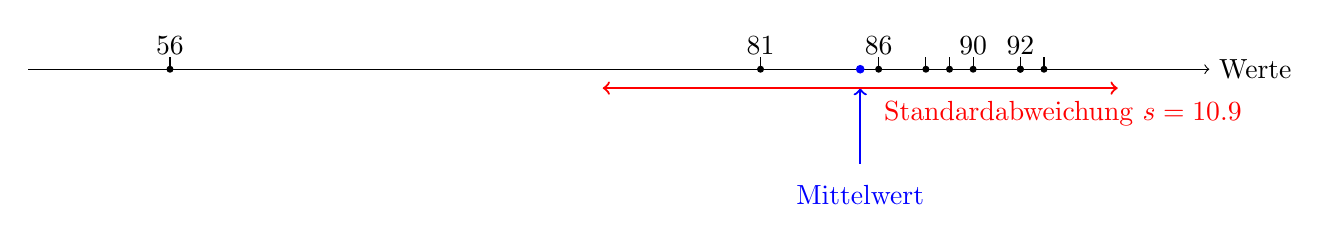
\begin{tikzpicture}[scale=0.3]
% Zahlenstrahl
\draw[->] (50,0) -- (100,0) node[right] {Werte};

% Ticks und Werte
\foreach \x in {56,81,86,88,89,90,92,93} {
  \draw (\x,0) -- (\x,0.5);
}

\foreach \x in {56,81,86,90,92} {
  \node[above] at (\x,0.2) {\x};
}

% Datenpunkte
\foreach \x in {56,81,86,88,89,90,92,92,93} {
  \filldraw[black] (\x,0) circle (3.5pt);
}

% Mittelwert
\filldraw[blue] (85.22,0) circle (4.5pt);
\draw[->, blue, thick] (85.22, -4) -- (85.22, -0.8);
\node[below, yshift=-1ex, text=blue] at (85.22, -4) {Mittelwert};

% Standardabweichungspfeile
\draw[<->, thick, red] (74.32, -0.8) -- (96.12, -0.8);
\node[above, text=red] at (93.8, -2.8) {Standardabweichung $s = 10.9$};

\end{tikzpicture}
\caption{Mittelwert und Standardabweichung auf dem Zahlenstrahl}
\end{figure}



\begin{aufgabe}{2}
Für die beiden Gruppen aus Aufgabe~1, berechnen Sie Varianz und Standardabweichung, und erklären Sie den Unterschied.
\begin{itemize}
\item \textbf{Gruppe A:} $[3,\ 4,\ 4,\ 4,\ 5,\ 6,\ 8]$
\item \textbf{Gruppe B:} $[3,\ 4,\ 5,\ 6,\ 7,\ 8,\ 20]$
\end{itemize}
\end{aufgabe}

Wir haben nun einige Lagekennwerte und einige Steuungsmasse kennengelernt. Mit diesen können wir, vereinfacht gesagt, ausdrücken, \textit{wo} sich ein Datensatz befindet, und die Varianz und Standardabweichung beschreiben, wie stark die Werte im Durchschnitt vom Mittelwert abweichen. Sie funktionieren besonders gut bei symmetrischen, ``glockenförmigen'' Verteilungen – wie sie in vielen physikalischen oder technischen Kontexten vorkommen.

Doch was, wenn die Verteilung \textbf{nicht symmetrisch} ist? (Zum Beispiel wie oben!) Oder wenn wir wissen möchten, \emph{welcher Anteil der Daten unterhalb oder oberhalb eines bestimmten Werts liegt}? Dann reichen Mittelwert und Standardabweichung oft nicht aus.

Hier kommen die \textit{Perzentile} ins Spiel: Sie geben an, wie gross der Anteil der Daten ist, der unterhalb eines bestimmten Werts liegt. Damit lässt sich etwa sagen:

\begin{itemize}
  \item ``75\% der Werte liegen unterhalb von $x$'' (das 75. Perzentil),
  \item ``die mittleren 50\% liegen zwischen dem 25. und 75. Perzentil'' (Interquartilsabstand).
\end{itemize}

Im Gegensatz zur Standardabweichung sind Perzentile robust gegenüber Ausreissern und funktionieren auch bei unsymmetrischen Verteilungen. Deshalb werden sie z. B. oft in der Medizin oder Soziologie verwendet, wo Extremwerte häufig sind.

\begin{aufgabe}{3}
Ein bestimmtes Perzentil, nämlich das \textit{50. Perzentil}, haben Sie in diesem Kapitel, allerdings unter einem anderen Namen, bereits kennengelernt: Wie nennt man den Wert, der so gelegen ist, dass 50\% (also die Hälfte) aller Werte darunter liegen?
\end{aufgabe}


\begin{theorie}
Mit \textbf{Perzentilen} können wir spezielle Werte in einer Gruppe bezeichnen. Diese sind speziell, weil sie genau so liegen, dass ein bestimmter Prozentsatz der Daten \emph{unterhalb} dieses Werts liegt.

\begin{itemize}
  \item Das \textbf{25. Perzentil} bedeutet: 25\,\% der Werte sind kleiner oder gleich diesem Wert.
  \item Das \textbf{90. Perzentil} bedeutet: 90\,\% der Werte liegen darunter.
\end{itemize}

\textbf{Quartile} sind spezielle Perzentile, die die Daten in vier gleich grosse Teile teilen:
\begin{itemize}
  \item $Q_1 =$ 25. Perzentil (unteres Quartil)
  \item $Q_2 =$ 50. Perzentil  (= Median)
  \item $Q_3 =$ 75. Perzentil (oberes Quartil)
\end{itemize}
\end{theorie}

Nehmen wir als Beispiel folgende Daten: $[56,\ 81,\ 86,\ 88,\ 89,\ 90,\ 92,\ 92,\ 93]$.

\begin{itemize}
  \item $Q_1 = 86$ → 25\,\% der Werte sind $\leq 86$
  \item $Q_2 = 89$ → 50\,\% der Werte sind $\leq 89$ (Median)
  \item $Q_3 = 92$ → 75\,\% der Werte sind $\leq 92$
\end{itemize}


\begin{aufgabe}{4}
Erweitern Sie die obige Zahlenreihe auf zehn Werte durch Hinzufügen von 94:

\[
[56,\ 81,\ 86,\ 88,\ 89,\ 90,\ 92,\ 92,\ 93,\ 94]
\]

Bestimmen Sie nun das 25., 50.\ (= Median) und 90. Perzentil.
\end{aufgabe}

\begin{aufgabe}{5*}
    Sie können diese neuen Begriffe mit \href{https://create.kahoot.it/share/statistics/5a4e45fc-22f3-4de5-920d-64aed3b9ffe0}{diesem \textit{kahoot}}\footnote{\href{https://create.kahoot.it/share/statistics/5a4e45fc-22f3-4de5-920d-64aed3b9ffe0}{\url{create.kahoot.it/share/statistics/5a4e45fc-22f3-4de5-920d-64aed3b9ffe0}}} üben. Wenn Sie diese LPU im Klassenverband bearbeiten, kann Ihre Lehrperson das \textit{kahoot} mit \tikz[baseline=(X.base)] 
  \node[draw=blue, very thick, rounded corners, inner xsep=2pt, inner ysep=4pt] 
  (X) {\textsf{Host live}}; für Ihre Klasse laufen lassen; ansonsten können Sie mit \tikz[baseline=(X.base)] 
  \node[draw=gray, very thick, rounded corners, inner xsep=2pt, inner ysep=4pt] 
  (X) {\textsf{Play solo}}; gefolgt von \tikz[baseline=(X.base)] 
  \node[draw=purple, very thick, rounded corners, inner xsep=2pt, inner ysep=4pt] 
  (X) {\textsf{Classic mode}}; alleine üben.
\end{aufgabe}

\subsection*{Zusammenfassung}
Wir sind nun an einem entscheidenden Punkt in dieser LPU angelangt: Sie haben drei grundlegende Algorithmen kennengelernt:

\begin{itemize}
  \item \textbf{Entscheidungsbaum:} Wenn das Ziel eine von mehreren vordefinierten Kategorien ist (z. B. ``spam'' oder ``kein spam'').
  \item \textbf{(Lineare) Regression:} Wenn das Ziel ein numerischer Wert ist, der geschätzt werden soll (z. B. Preis, Temperatur, Dauer).
  \item \textbf{\textit{k-means}:} Wenn es kein Zielattribut gibt und Sie Gruppen aus ähnlichen Datenpunkten automatisch erkennen möchten.
\end{itemize}

Alle drei Algorithmen können mit numerischen und kategorischen Eingabedaten umgehen. Entscheidend ist, \emph{welche Art von Aufgabe} gelöst werden soll.

\begin{aufgabe}{6}
Öffnen Sie Ihr Glossardokument und ergänzen Sie folgende Begriffe mit einer eigenen Definition:

\begin{itemize}
  \item decision tree (Entscheidungsbaum)
  \item linear regression (lineare Regression)
  \item \textit{k-means}
\end{itemize}

Überdenken Sie auch frühere Begriffsdefinitionen: Haben sich durch die neuen Aufträge Ihre Formulierungen verändert?
\end{aufgabe}
\end{lpu}


\subsection*{Didaktische Überlegungen}

Statistik bildet das Fundament datengetriebener Verfahren – auch und gerade im maschinellen Lernen. Dennoch ist Statistik unter SuS oft mit Vorurteilen belegt: ``zu abstrakt'', ``zu trocken'', ``zu mathematisch''. Um diese Barrieren abzubauen, wurde das Kapitel bewusst \textbf{nicht an den Anfang} der LPU gesetzt, obwohl es inhaltlich auch dort hätte stehen können.

Nach Kapiteln zu Entscheidungsbäumen, Regression und Clustering haben die SuS bereits erlebt, \emph{was mit Daten möglich ist}: Vorhersagen treffen, Gruppen erkennen, Modelle evaluieren. Sie haben mit echten Datensätzen gearbeitet und eigene Vermutungen überprüfen können. Diese positiven Erfahrungen schaffen eine Offenheit gegenüber den ``Werkzeugen im Hintergrund'', also den statistischen Begriffen, mit denen man Daten sinnvoll beschreiben kann. Beim Arrangieren dieser LPU habe ich mich diesbezüglich also an der Formel \emph{Zuerst erleben, dann erklären} orientiert.

Besonders hilfreich scheinen mir die Aufgaben, in denen die SuS mehrere Gruppen vergleichen, z. B. mit ähnlichem Mittelwert, aber unterschiedlicher Streuung. Dadurch entsteht ein intuitives Verständnis für die Begriffe \emph{Lage} und \emph{Streuung}, das weit über formales Rechnen hinausgeht.

Ein besonderer didaktischer Akzent liegt auf dem abschliessenden \textit{kahoot}-Quiz. Dieses Format bringt Bewegung, Energie und einen spielerischen Zugang zum Stoff – besonders in einem Kapitel, das potenziell ``kopflastig'' wirken könnte. Es erstaunt mich jedes Mal wieder auf's Neue, wie einfach es ist, die SuS mit \textit{kahoot} zum Mitmachen zu bewegen.

Das Quiz kann aber auch inhaltlich vertieft werden: Die SuS erhalten am Ende eine Punktzahl und eine Platzierung. Diese kann direkt genutzt werden, um Perzentile praktisch zu erklären:

\begin{itemize}
  \item ``Du bist im 80. Perzentil – 80\,\% der Klasse hatten weniger Punkte als du.''
  \item ``Das 50. Perzentil lag bei 9 Punkten – das war der Median der Runde.''
\end{itemize}

So werden statistische Begriffe mit unmittelbarer Erfahrung verknüpft – und das nicht in einem bewertenden, sondern spielerischen Rahmen. 

Im abschliessenden Teil dieses Kapitels liegt der Fokus auf der Unterscheidung von Algorithmen. Dieser Abschnitt ermöglicht eine rückblickende Konsolidierung: Die SuS fassen nochmals zusammen, welche Verfahren sie kennengelernt haben (Entscheidungsbaum, Regression, Ballung) und wann man sie jeweils sinnvoll einsetzt.

Die Glossaraufgabe zielt dabei auf eine \textbf{Meta-Ebene des Lernens}: SuS überarbeiten frühere Definitionen, verbessern ihre Sprache und verankern die Begriffe im eigenen Sprachgebrauch. Dies unterstützt die semantische Klarheit und die Fähigkeit zur selbstständigen Anwendung.

Dieses Kapitel ist also ein Scharnierkapitel: Es verbindet erlebtes maschinelles Lernen mit den zugrunde liegenden Konzepten der Statistik – und bereitet zugleich den Boden für die kritische Anwendung und Evaluation von Modellen.





\subsection*{Musterlösungen}

\begin{aufgabe}{1}
\textbf{Gegeben:}

\begin{itemize}
  \item \textbf{Gruppe A:} $[3,\ 4,\ 4,\ 4,\ 5,\ 6,\ 8]$
  \begin{itemize}
    \item Mittelwert: $\bar{x}_A = \frac{3 + 4 + 4 + 4 + 5 + 6 + 8}{7} = \frac{34}{7} \approx 4.86$
    \item Median: Der 4. Wert (zentraler Wert): $4$
    \item Modus: Der häufigste Wert ist $4$
  \end{itemize}
  \item \textbf{Gruppe B:} $[3,\ 4,\ 5,\ 6,\ 7,\ 8,\ 20]$
  \begin{itemize}
  \item Mittelwert: $\bar{x}_B = \frac{3 + 4 + 5 + 6 + 7 + 8 + 20}{7} = \frac{53}{7} \approx 7.57$
  \item Median: Der 4. Wert (zentraler Wert): $6$
  \item Modus: Kein Wert kommt doppelt vor $\Rightarrow$ kein Modus
\end{itemize}
\end{itemize}

Manche statistische Programme geben in solchen Fällen wie hier bei Gruppe B den Modus als ``nicht definiert'' oder ``mehrdeutig'' aus. Als plausible Alternative kann man hier auch sagen: ``Gruppe B hat keinen \textit{eindeutigen} Modus.''

Die nachfolgende Visualisierung zeigt deutlich, dass der Mittelwert von Gruppe B nach rechts ``gezogen'' wird – durch den Ausreisser $20$.

\begin{figure}[H]
\centering
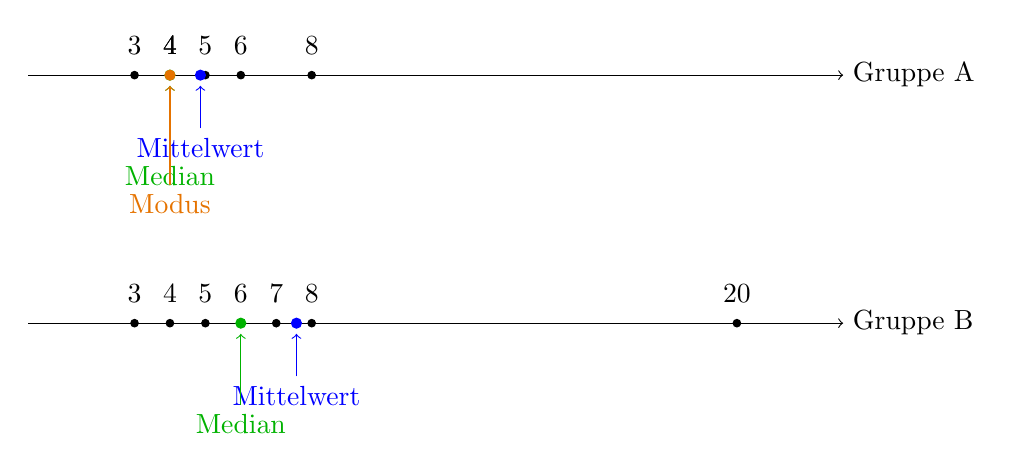
\begin{tikzpicture}[scale=0.45]
% Zahlenstrahle
\draw[->] (0,0) -- (23,0) node[right] {Gruppe A};
\draw[->] (0,-7) -- (23,-7) node[right] {Gruppe B};

% Gruppe A: Punkte
\filldraw[black] (3,0) circle (3pt);
\filldraw[black] (4,0) circle (3pt);
\filldraw[black] (4,0) circle (3pt);
\filldraw[black] (4,0) circle (3pt);
\filldraw[black] (5,0) circle (3pt);
\filldraw[black] (6,0) circle (3pt);
\filldraw[black] (8,0) circle (3pt);

% Gruppe A: Mittelwert
\filldraw[blue] (4.86,0) circle (4pt);
\draw[->, blue] (4.86, -1.5) -- (4.86, -0.3);
\node[below, text=blue] at (4.86, -1.5) {Mittelwert};

% Gruppe A: Median
\filldraw[green!70!black] (4,0) circle (4pt);
\draw[->, green!70!black] (4, -2.3) -- (4, -0.3);
\node[below, text=green!70!black] at (4, -2.3) {Median};

% Gruppe A: Modus
\filldraw[orange!90!black] (4,0) circle (4pt);
\draw[->, orange!90!black] (4, -3.1) -- (4, -0.3);
\node[below, text=orange!90!black] at (4, -3.1) {Modus};

% Gruppe B: Punkte
\filldraw[black] (3,-7) circle (3pt);
\filldraw[black] (4,-7) circle (3pt);
\filldraw[black] (5,-7) circle (3pt);
\filldraw[black] (6,-7) circle (3pt);
\filldraw[black] (7,-7) circle (3pt);
\filldraw[black] (8,-7) circle (3pt);
\filldraw[black] (20,-7) circle (3pt);

% Gruppe B: Mittelwert
\filldraw[blue] (7.57,-7) circle (4pt);
\draw[->, blue] (7.57, -8.5) -- (7.57, -7.3);
\node[below, text=blue] at (7.57, -8.5) {Mittelwert};

% Gruppe B: Median
\filldraw[green!70!black] (6,-7) circle (4pt);
\draw[->, green!70!black] (6, -9.3) -- (6, -7.3);
\node[below, text=green!70!black] at (6, -9.3) {Median};

% Beschriftungen Gruppe A
\node[above] at (3,0.3) {3};
\node[above] at (4,0.3) {4};
\node[above] at (4,0.3) {4};
\node[above] at (4,0.3) {4};
\node[above] at (5,0.3) {5};
\node[above] at (6,0.3) {6};
\node[above] at (8,0.3) {8};

% Beschriftungen Gruppe B
\node[above] at (3,-6.7) {3};
\node[above] at (4,-6.7) {4};
\node[above] at (5,-6.7) {5};
\node[above] at (6,-6.7) {6};
\node[above] at (7,-6.7) {7};
\node[above] at (8,-6.7) {8};
\node[above] at (20,-6.7) {20};
\end{tikzpicture}
\caption{Vergleich der drei M bei Gruppe A und Gruppe B}
\end{figure}



\begin{itemize}
  \item \textbf{Was unterscheidet die beiden Gruppen?}

  Gruppe A ist relativ symmetrisch und kompakt um den Wert $4$ verteilt. Gruppe B enthält einen Ausreisser ($20$), der weit vom restlichen Zentrum entfernt liegt. Dadurch verändert sich der Mittelwert stark.

  \item \textbf{Welcher Lagekennwert ist besonders empfindlich gegenüber Ausreissern?}

  Der \textbf{Mittelwert} ist empfindlich gegenüber Ausreissern: In Gruppe B steigt er von $\approx 4.86$ auf $\approx 7.57$, obwohl sich nur ein einziger Wert geändert hat. Median und Modus bleiben stabil oder verändern sich wenig.

  \item \textbf{Warum nennt man diese Werte ``Lagekennwerte''? Was ist ihre ``Lage''?}

  Diese Werte geben an, \emph{wo} sich die Daten im Zahlenraum befinden. Sie beschreiben die typische Position der Werte – also ihre ``Lage'' auf dem Zahlenstrahl. Dabei betonen sie jeweils unterschiedliche Aspekte:

  Sie helfen dabei, eine Zahlenreihe auf einen einzigen ``repräsentativen'' Wert zu reduzieren – je nach Fragestellung auf unterschiedliche Weise.
\end{itemize}
\end{aufgabe}

\begin{aufgabe}{2}

Gegeben:

\begin{itemize}
  \item \textbf{Gruppe A:} $[3,\ 4,\ 4,\ 4,\ 5,\ 6,\ 8]$
  \item \textbf{Gruppe B:} $[3,\ 4,\ 5,\ 6,\ 7,\ 8,\ 20]$
\end{itemize}

Für $n$ Werte $x_1, x_2, \dots, x_n$ mit Mittelwert $\bar{x}$ gilt:

\[
s^2 = \frac{1}{n} \sum_{i=1}^{n} (x_i - \bar{x})^2 \qquad \text{(Varianz)}
\]
\[
s = \sqrt{s^2} \qquad \text{(Standardabweichung)}
\]

\textbf{Gruppe A:}

\[
\bar{x}_A = \frac{3 + 4 + 4 + 4 + 5 + 6 + 8}{7} = \frac{34}{7} \approx 4.86
\]

\[
s^2_A = \frac{1}{7} \big((3-4.86)^2 + (4-4.86)^2 + (4-4.86)^2 + (4-4.86)^2 + (5-4.86)^2 + (6-4.86)^2 + (8-4.86)^2\big) \approx 2.12
\]

\[
s_A = \sqrt{2.12} \approx 1.46
\]

\textbf{Gruppe B:}

\[
\bar{x}_B = \frac{3 + 4 + 5 + 6 + 7 + 8 + 20}{7} = \frac{53}{7} \approx 7.57
\]

\[
s^2_B = \frac{1}{7} \big((3-7.57)^2 + (4-7.57)^2 + (5-7.57)^2 + (6-7.57)^2 + (7-7.57)^2 + (8-7.57)^2 + (20-7.57)^2\big) \approx 28.39
\]

\[
s_B = \sqrt{28.39} \approx 5.33
\]

\textbf{Varianz} misst, wie stark die Daten im Durchschnitt vom Mittelwert abweichen – allerdings in \emph{quadratischen Einheiten}. Deshalb ist sie gut mathematisch verwendbar, aber weniger anschaulich.

\textbf{Standardabweichung} ist die ``normale'' Streuung der Werte um den Mittelwert, wieder in den \emph{gleichen Einheiten wie die Daten}. Sie ist deshalb leichter interpretierbar.

\begin{itemize}
  \item Gruppe A ist kompakt um den Mittelwert 4.86 verteilt. Die Abweichungen sind klein und relativ symmetrisch.
  \item Gruppe B enthält den Ausreisser $20$. Dieser liegt weit rechts vom Zentrum und erhöht sowohl Mittelwert als auch Streuung massiv.
\end{itemize}

Standardabweichung ist also stark empfindlich gegenüber Ausreissern – sie ``sieht'' den Ausreisser sofort.

\end{aufgabe}

\begin{aufgabe}{3}

\textbf{Frage:} Wie nennt man den Wert, unter dem 50 \% aller Werte liegen?
\textbf{Antwort:} Diesen Wert nennt man den \textbf{Median}.

\textbf{Begründung:} Der Median ist per Definition der Wert, der die sortierte Datenmenge in zwei gleich grosse Hälften teilt:

\begin{itemize}
  \item 50 \% der Werte liegen unterhalb (oder gleich) dem Median,
  \item 50 \% der Werte liegen oberhalb (oder gleich) dem Median.
\end{itemize}

Man bezeichnet den Median daher auch als \textbf{das 50. Perzentil}.

\textbf{Didaktische Weiterführung:} Diese Aufgabe eignet sich gut, um den Zusammenhang zwischen \textbf{Perzentilen} und \textbf{Lagekennwerten} zu verdeutlichen. Die SuS erkennen hier:

\begin{itemize}
  \item Der Median ist ein \emph{spezialisiertes Perzentil} (nämlich das 50.).
  \item Andere Perzentile wie das 25. ($Q_1$) oder das 75. ($Q_3$) sind ebenfalls leicht interpretierbar.
\end{itemize}

\end{aufgabe}

\begin{aufgabe}{4}

\textbf{Gegebene Datenreihe (sortiert):}
\[
[56,\ 81,\ 86,\ 88,\ 89,\ 90,\ 92,\ 92,\ 93,\ 94]
\]

\textbf{Anzahl der Werte:} $n = 10$

Das 25. Perzentil liegt bei Position:
\[
P = 0.25 \cdot (n + 1) = 0.25 \cdot 11 = 2.75
\]

Dieser Wert liegt zwischen dem 2. und 3. Wert, bei 75 \% zwischen 81 und 86:

\[
P_{25} = 81 + 0.75 \cdot (86 - 81) = 81 + 3.75 = \boxed{84.75}
\]

Bei gerader Anzahl $n = 10$ liegt der Median zwischen dem 5. und 6. Wert:

\[
P_{50} = \frac{89 + 90}{2} = \boxed{89.5}
\]

Für das 90. Perzentil:

\[
P = 0.90 \cdot (n + 1) = 0.90 \cdot 11 = 9.9
\]

→ Position zwischen 9. und 10. Wert, bei 90 \% zwischen 93 und 94:

\[
P_{90} = 93 + 0.9 \cdot (94 - 93) = 93 + 0.9 = \boxed{93.9}
\]

\textbf{Hinweis für die Praxis:} Viele Softwarepakete (z. B. Excel, Python, R) verwenden leicht unterschiedliche Verfahren zur Interpolation. Wichtig ist daher das methodische Grundverständnis – nicht eine exakte Zahl auf vier Nachkommastellen.

\end{aufgabe}

\begin{aufgabe}{6} Folgendes sind Beispiel-Einträge:

\begin{itemize}
  \item \textbf{decision tree (Entscheidungsbaum):}  
  Ein Entscheidungsbaum ist ein Modell, das Daten durch binäre Fragen schrittweise aufteilt, um am Ende zu einer Entscheidung zu kommen. Jeder Ast steht für eine Entscheidung, und jedes Blatt für ein Ergebnis. Der Baum kann verwendet werden, um neue Fälle automatisch zu klassifizieren.

  \item \textbf{linear regression (lineare Regression):}  
  Ein mathematisches Modell, das eine Gerade so durch eine Punktwolke legt, dass sie möglichst gut zu den Daten passt. Damit kann man Vorhersagen machen: z. B. wie gross etwas wahrscheinlich ist, wenn man einen bestimmten Wert kennt.

  \item \textbf{k-means:}  
  Ein Verfahren, das Daten in Gruppen unterteilt, ohne dass diese vorher festgelegt sind. Der Algorithmus sucht automatisch Gruppen, indem er Punkte nach ihrer Nähe zu Gruppenzentren zusammenfasst. Diese Zentren werden so lange angepasst, bis sich nichts mehr verändert.
\end{itemize}

\end{aufgabe}

Diese Glossaraufgabe eignet sich gut zur Wiederholung und Selbstvergewisserung; und kann zu Beginn einer Lektion eingesetzt werden. Man kann die SuS auch gegenseitig ihre Einträge vergleichen und diskutieren lassen, um Begriffssicherheit aufzubauen.